\documentclass[main.tex]{subfiles}
 
\begin{document}

\part{Slow slip}

\chapter{Data}

The data are available on the website of the Pacific Northwest Geodetic Array (\href{http://www.geodesy.cwu.edu/}{PANGA}), from Central Washington University. Three types of time series are available:

\begin{itemize}
\item Raw data recorded by the GPS stations, after GIPSY postprocessing.
\item Detrended data, for which a linear trend corresponding to the secular plate motion has been removed from the data.
\item Cleaned data, for which the linear trend, steps due to earthquakes or hardware upgrades, and annual and semi-annual sinusoids signals have been simultaneously estimated and removed following Szeliga \textit{et al.} (2008 ~\cite{SZE_2008}).
\end{itemize}

For each GPS station, the website provides a file for the three components of the displacement (latitude, longitude, and vertical), and each file contains three columns, corresponding to the time, the displacement (in millimetres), and the error. The data are recorded once a day. \\

The data are filtered with the function $f (t)$:

\begin{equation}
f (t) = \textrm{line} (t) + \textrm{annual} (t) + \textrm{jumps} (t)
\end{equation}

with:

\begin{equation}
\textrm{line} (t) = p_1 + p_2 t
\end{equation}

\begin{equation}
\textrm{annual} (t) = p_3 \sin (2 \pi t + p_4) + p_5 \sin (4 \pi t + p_6)
\end{equation}

\begin{equation}
\textrm{jumps} (t) = \sum_{i = 1}^{n} p_i \textrm{Heaviside} (t - t_i)
\end{equation}

The values of the $p_i$ and $t_i$ are given at the beginning of each file.

Add something about the inversion of these parameters (Nikolaidis, 2002), and about the seasonal trends (Blewitt and Lavall\'ee, 2002)). 

\chapter{Method}

The Discrete Wavelet Transform (DWT) is an orthonormal transform that associates a time series $X_t (t = 0 , ... , N - 1)$ written in the traditional orthonormal basis:

\begin{equation}
\bm{X} = X_0 \begin{pmatrix} 1 \\ 0 \\ 0 \\ . \\ . \\ . \\ 0 \end{pmatrix}
+ X_1 \begin{pmatrix} 0 \\ 1 \\ 0 \\ . \\ . \\ . \\ 0 \end{pmatrix}
+ X_2 \begin{pmatrix} 0 \\ 0 \\ 1 \\ . \\ . \\ . \\ 0 \end{pmatrix}
+ ... + X_{N - 1} \begin{pmatrix} 0 \\ 0 \\ 0 \\ . \\ . \\ . \\ 1 \end{pmatrix}
\end{equation}

into the same times series written in another orthonormal basis:

\begin{equation}
X = W_0 \begin{pmatrix} \mathcal{W}_{0 , 0} \\ \mathcal{W}_{0 , 1} \\ \mathcal{W}_{0 , 2} \\ . \\ . \\ . \\ \mathcal{W}_{0 , N - 1} \end{pmatrix}
+ W_1 \begin{pmatrix} \mathcal{W}_{1 , 0} \\ \mathcal{W}_{1 , 1} \\ \mathcal{W}_{1 , 2} \\ . \\ . \\ . \\ \mathcal{W}_{1 , N - 1} \end{pmatrix}
+ W_2 \begin{pmatrix} \mathcal{W}_{2 , 0} \\ \mathcal{W}_{2 , 1} \\ \mathcal{W}_{2 , 2} \\ . \\ . \\ . \\ \mathcal{W}_{2 , N - 1} \end{pmatrix}
+ ... + W_{N - 1} \begin{pmatrix} \mathcal{W}_{N - 1 , 0} \\ \mathcal{W}_{N - 1 , 1} \\ \mathcal{W}_{N - 1 , 2} \\ . \\ . \\ . \\ \mathcal{W}_{N - 1 , N - 1} \end{pmatrix}
\end{equation}

where the $\mathcal{W}_{i , .}$ are the wavelet basis vectors.

The first $\frac{N}{2}$ $\mathcal{W}_{i , .}$ vectors are circularly shifted with each other:

\begin{equation}
\mathcal{W}_{k , j} = \mathcal{W}_{i , j + 2 \left( i - k \right)}
\end{equation}

and their Fourier transform has a nominal frequency band of $\lbrack \frac{1}{4 dt} ; \frac{1}{2 dt} \rbrack$.

We can write $\mathcal{W}_{i , j} = h_{2 i + 1 - j \mod N}$, where $h_l \left( l = 0 , ... , N - 1 \right)$ is the wavelet filter.

The next $\frac{N}{4}$ $\mathcal{W}_{i , .}$ vectors are also circularly shifted with each other:

\begin{equation}
\mathcal{W}_{k , j} = \mathcal{W}_{i , j + 4 \left( i - k \right)}
\end{equation}

and their Fourier transform has a nominal frequency band of $\lbrack \frac{1}{8 dt} ; \frac{1}{4 dt} \rbrack$.

We can write $\mathcal{W}_{i , j} = \sum_{l = 0}^{N - 1} g_{l - j} h_{4 i + 3 - l \mod N}^{\uparrow}$, where $h_l^{\uparrow}$ is formed by inserting a $0$ between each of the elements of $h_l$, and $g_l \left( l = 0 , ... , N - 1 \right)$ is the scaling filter defined by:

\begin{equation}
g_l = \left( - 1 \right) ^{l + 1} h_{N - 1 - l}
\end{equation}

At the level $J$, we can write the orthonormal transform as:

\begin{equation}
W = \mathcal{W} X \text{ or } \begin{pmatrix} W_1 \\ W_2 \\ W_3 \\ . \\ . \\ . \\ W_J \\ V_J \end{pmatrix}
= \begin{pmatrix} \mathcal{W}_1 X \\ \mathcal{W}_2 X \\ \mathcal{W}_3 X \\ . \\ . \\ . \\ \mathcal{W}_J X \\ \mathcal{V}_J X \end{pmatrix}
\end{equation}

Each of the wavelet vectors $W_j$ has length $\frac{N}{2^j}$, has a time step of $2^j dt$, and corresponds to the filtering of the initial time series by a filter of nominal frequency band $\lbrack \frac{1}{dt 2^{j + 1}} ; \frac{1}{dt 2^j} \rbrack$. The scaling vector $V_J$ has length $\frac{N}{2^J}$, has a time step of $2^J dt$, and corresponds to the filtering of the initial time series by a filter of nominal frequency band $\lbrack 0 ; \frac{1}{dt 2^{J + 1}} \rbrack$.

We can then compute the $j$th level detail $D_j \left( j = 1 , ... , J \right)$, which is a vector of length $N$, defined by $D_j = \mathcal{W}_j^T W_j$ and the $J$th level smooth $S_J$, which is a vector of length $N$, defined by $S_J = \mathcal{V}_j^T V_j$, and we get the multiresolution analysis (MRA) of $X$:

\begin{equation}
X = \sum_{j = 1}^{J} D_j + S_J
\end{equation}

If we want to keep the length $N$ and the time step $dt$ of $X$, we can use a modification of the DWT, the Maximum Overlap Discrete Wavelet Transform (MODWT). The MODWT transforms the time series $X_t \left( t = 0, ... , N - 1 \right)$ into J wavelet vectors $\widetilde{W}_j \left( j = 1 , ... , J \right)$ of length $N$ and a scaling vector $\widetilde{V}_J$ of length $N$. Each wavelet vector $\widetilde{W}_j$ corresponds to the filtering of the original time series with a filter with nominal frequency band $\lbrack \frac{1}{dt 2^{j + 1}} ; \frac{1}{dt 2^j} \rbrack$. The scaling vector $\widetilde{V}_J$ corresponds to the filtering of the original time series with a filter with nominal frequency interval $\lbrack 0 ; \frac{1}{dt 2^{j + 1}} \rbrack$.

We can write the transformation as:

\begin{equation}
\widetilde{W}_j = \widetilde{\mathcal{W}_j} X \text{ and } \widetilde{V}_J = \widetilde{\mathcal{V}_J} X
\end{equation}

$ \widetilde{\mathcal{W}_j}$ and $\widetilde{\mathcal{V}_J}$ are related to $\mathcal{W}_j$ and $\mathcal{V}_J$ by:

\begin{equation}
\widetilde{\mathcal{W}}_{j, t l} = \widetilde{h}_{j , t - l \mod N} \text{, } \mathcal{W}_{j, t l} = h_{j , 2^j \left( t + 1 \right) - 1 - l \mod N} \text{ and } \widetilde{h}_{j , l} = \frac{h_{j , l}}{2^{j/2}}
\end{equation}

\chapter{Results}

In the following analysis, we used the cleaned dataset in order to minimize the discontinuity between the beginning and the end of the time series. In order to analyze the temporal correlation of the slow slip with the tremor, we also used the tremor catalog of the PNSN (Wech, 2010 ~\cite{WEC_2010}) to get the cumulative number of tremor recorded around the GPS station. The displacement is recorded once a day at every GPS station. However, there are many missing data points. We chose the GPS station PGC5, located in southern Vancouver Island, near Victoria. The slow slip events are clearly visible in the longitudinal component of the displacement (see bottom panel of Figure 19.1). Moreover, there are very few missing data for this station. In the following, we have analyzed eight years of GPS data from 2006 to 2014. There are only five days for which the displacement is missing. We replaced the missing data by the average of the displacement on the day before and the displacement on the day after. \\

We first carried out a partial DWT of the time series. To choose the appropriate wavelet filter, we computed the Normalized Partial Energy Sequence (NPES) of the wavelet coefficients and of the time series for different wavelet filters. It did not seem that there was much difference between the different wavelet filters. In the following, we will compare the wavelet coefficients to the cumulative number of tremor recorded around the GPS station. Therefore, we would like to know with good precision the time shift that should be applied to the wavelet coefficients. Moreover, we would like the length of the wavelet filter to remain small, in order to reduce the number of coefficients that are affected by the interpolation we had to do to replace the missing data. This is why we chose the LA8 wavelet filter in the following analysis. \\

The total duration of a slow slip event is about six weeks. Therefore, we only carried out a partial DWT up to the level 6 (corresponding to a scale of 64 days), because we do not expect to see features at a longer scale in the time series. \\

The wavelet coefficients for level 1 to 6 are shown in Figure 19.1. The red bars correspond to the days where data were missing. The grey bars correspond to the timing of ETS events.  We can clearly see big wavelet coefficients corresponding to the January 2007 ETS event at the levels 5 and 6, to the May 2009 ETS event at the level 5, to the August 2010 ETS event at the level 6, to the September 2012 ETS event at the levels 5 and 6, and to the September 2013 ETS event at the levels 5 and 6.  The May 2008 and August 2011 ETS events are not clearly seen in the wavelet coefficients. \\

\begin{center}
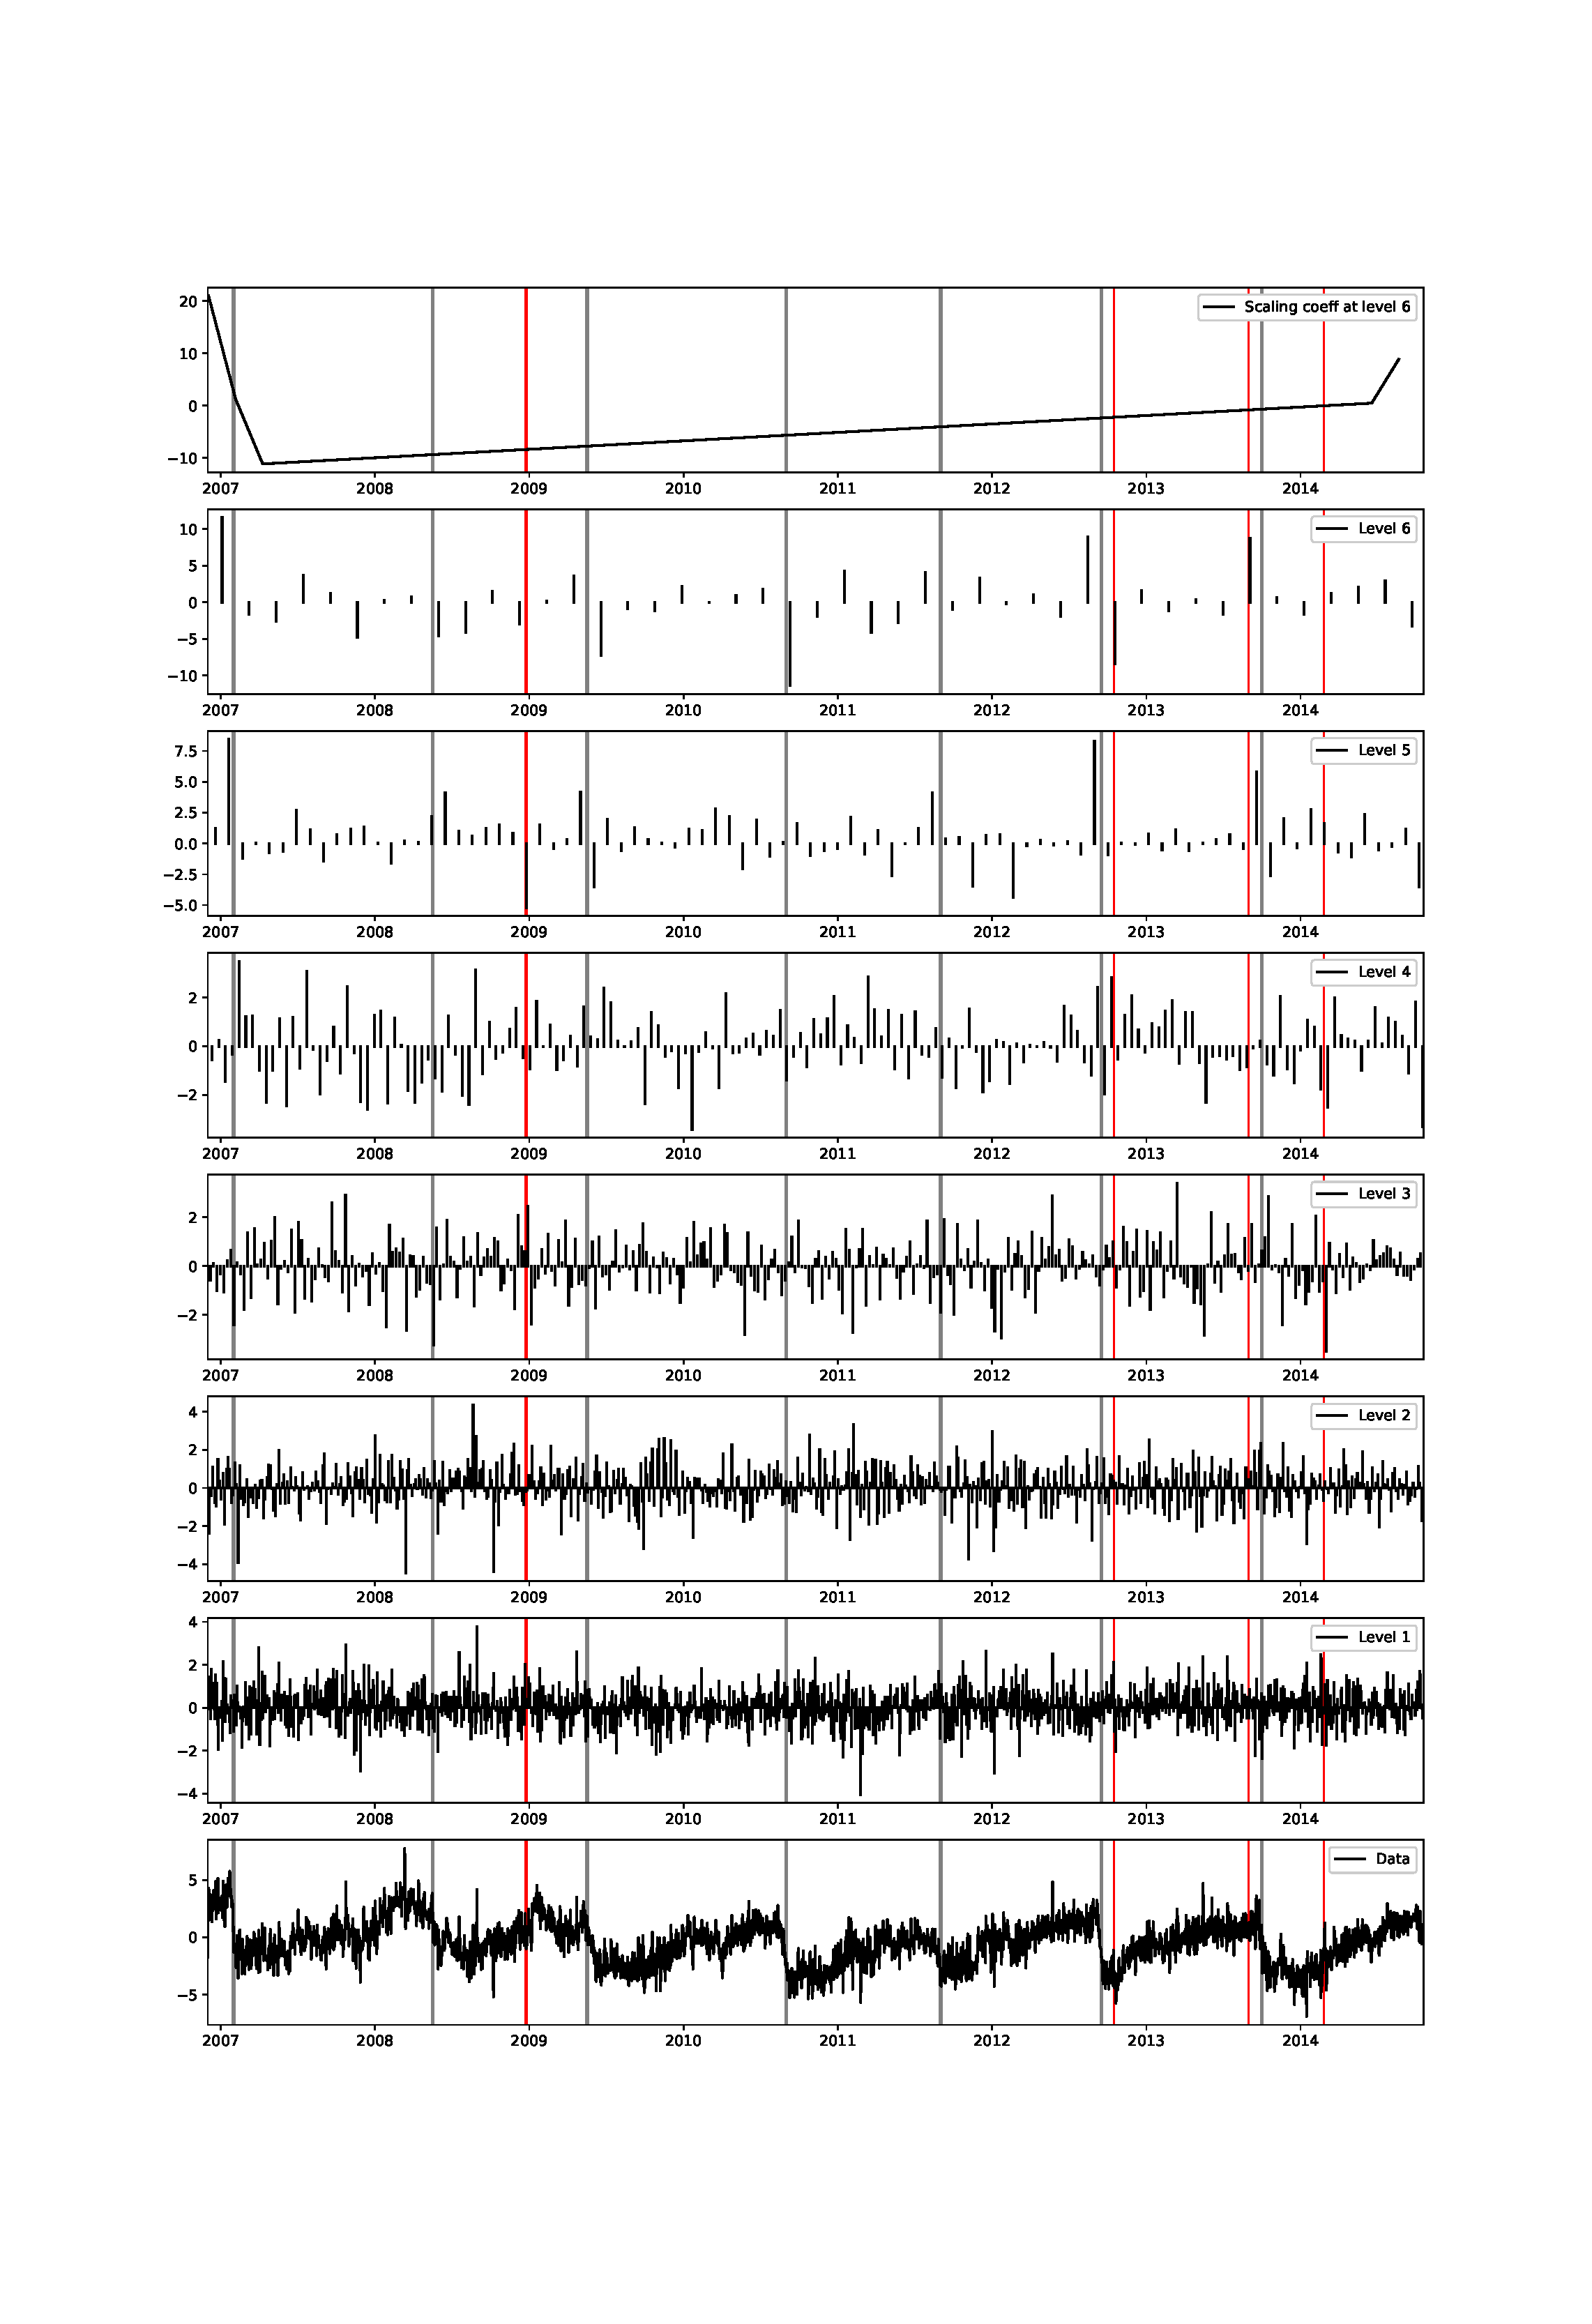
\includegraphics[width=300pt]{Figures/slowslip_results/Figure_1.eps}
\captionsetup{type=figure}
\captionof{figure}{Partial DWT wavelet coefficients up to level 6.}
\end{center}

Finally, the 5\textsuperscript{th} and 6\textsuperscript{th} level details of the MRA are plotted with the cumulative number of tremor in Figure 19.2. Unfortunately, the tremor catalog from the PNSN website only starts in August 2009. As the GPS station is located at latitude N48\degree39', we only took into account the tremor which source was located between latitude N47.5\degree and latitude N49.5\degree. We can clearly see the August 2010, September 2012 and September 2013 ETS events in the 6\textsuperscript{th} level detail. The August 2010 ETS event is less obvious, but can be seen in the 5\textsuperscript{th} level detail. There is a small increase in the number of tremor in March 2010, but is not really clear that there is a corresponding peak in the 5\textsuperscript{th} detail.

\begin{center}
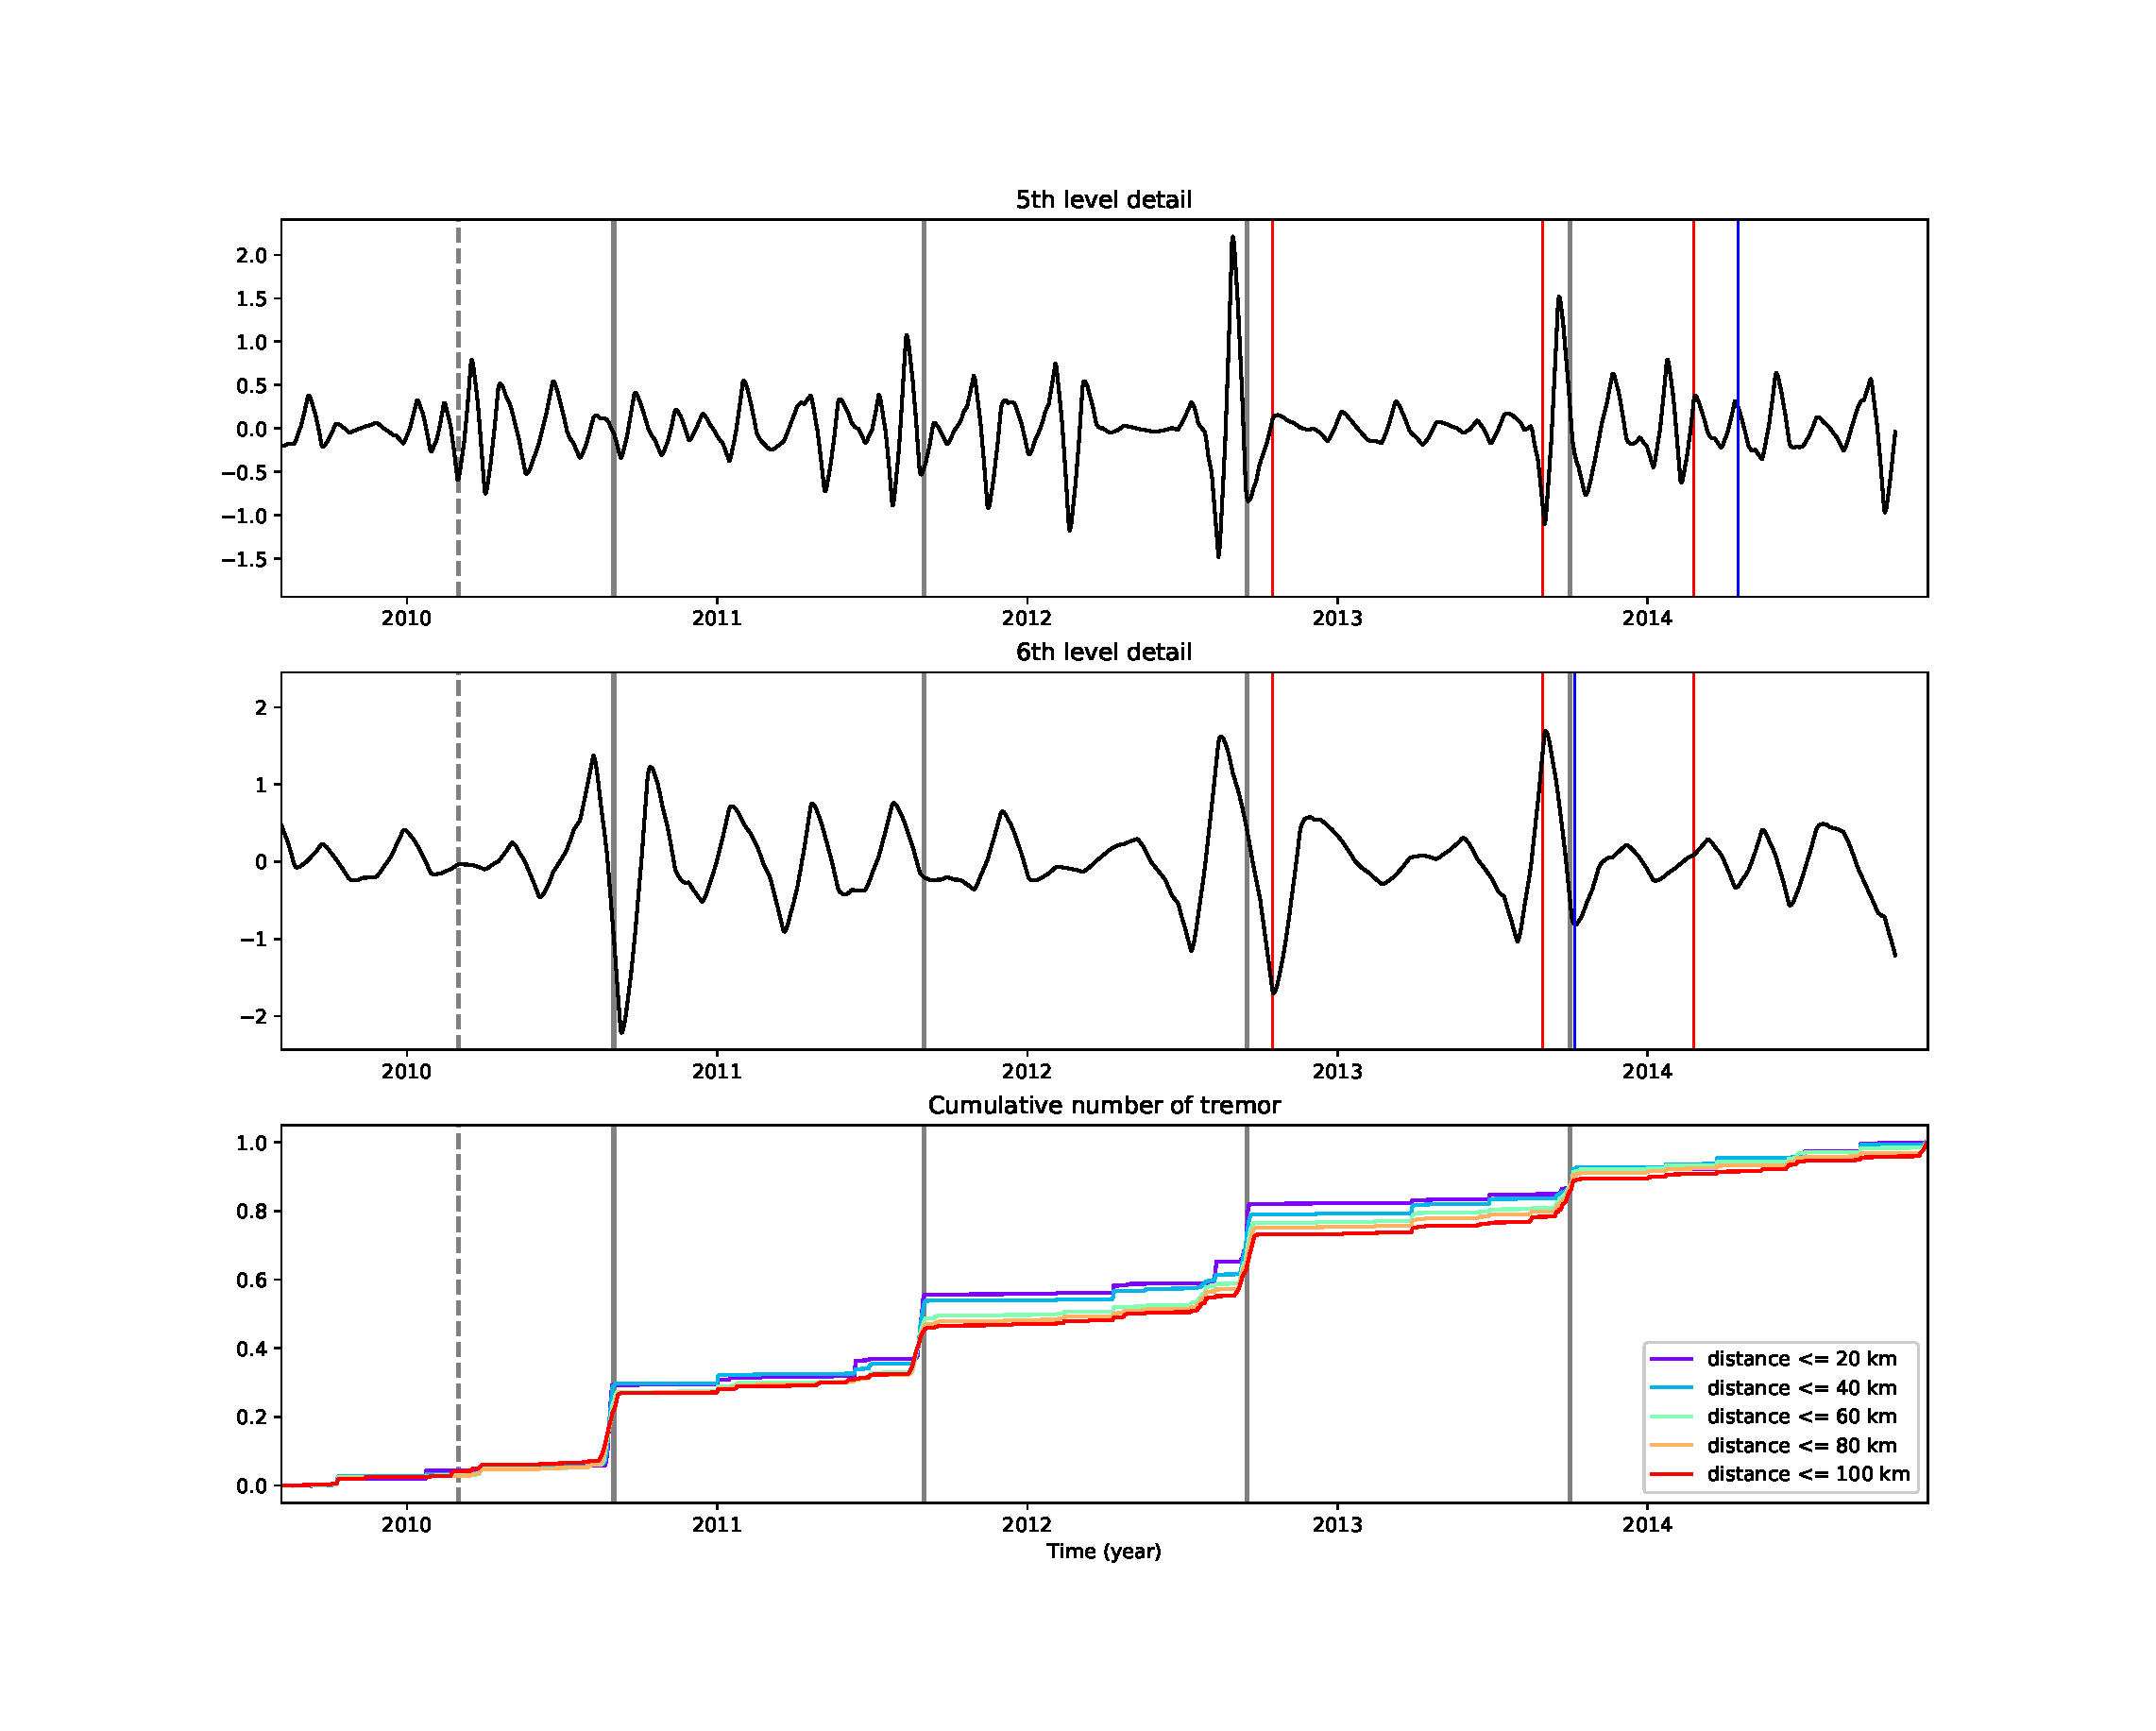
\includegraphics[width=300pt]{Figures/slowslip_results/Figure_2.eps}
\captionsetup{type=figure}
\captionof{figure}{5\textsuperscript{th} and 6\textsuperscript{th} level details of the partial DWT analysis (top and middle panel), and cumulative number of tremor
recorded around the GPS station (bottom panel).}
\end{center}

The details of the MRA with the partial DWT have a somewhat 'shark fin' look, which is not entirely pleasing. Moreover, the number of days between two ETS events may not correspond to a multiple of a power of 2. Therefore, it would be easier to interpret the wavelet coefficients at each level if their dimensions was the same as the dimension of the original time series. Finally, it would be easier to associate the details and smooths of the MRA with the cumulative number of tremor recorded if they were associated with zero phase filters. Therefore, in the following, we carried out a MODWT analysis on the same time series. \\

The wavelet coefficients for level 1 to 6 are shown in Figure 19.3. We can clearly see peaks corresponding to the January 2007, May 2009, August 2010, September 2012, and September 2013 ETS events in both the level 5 and level 6 coefficients. A peak corresponding to the May 2008 ETS event can be seen in the level 5 coefficients. However, it is still difficult to observe the August 2011 ETS event in the wavelet coefficients. \\

\begin{center}
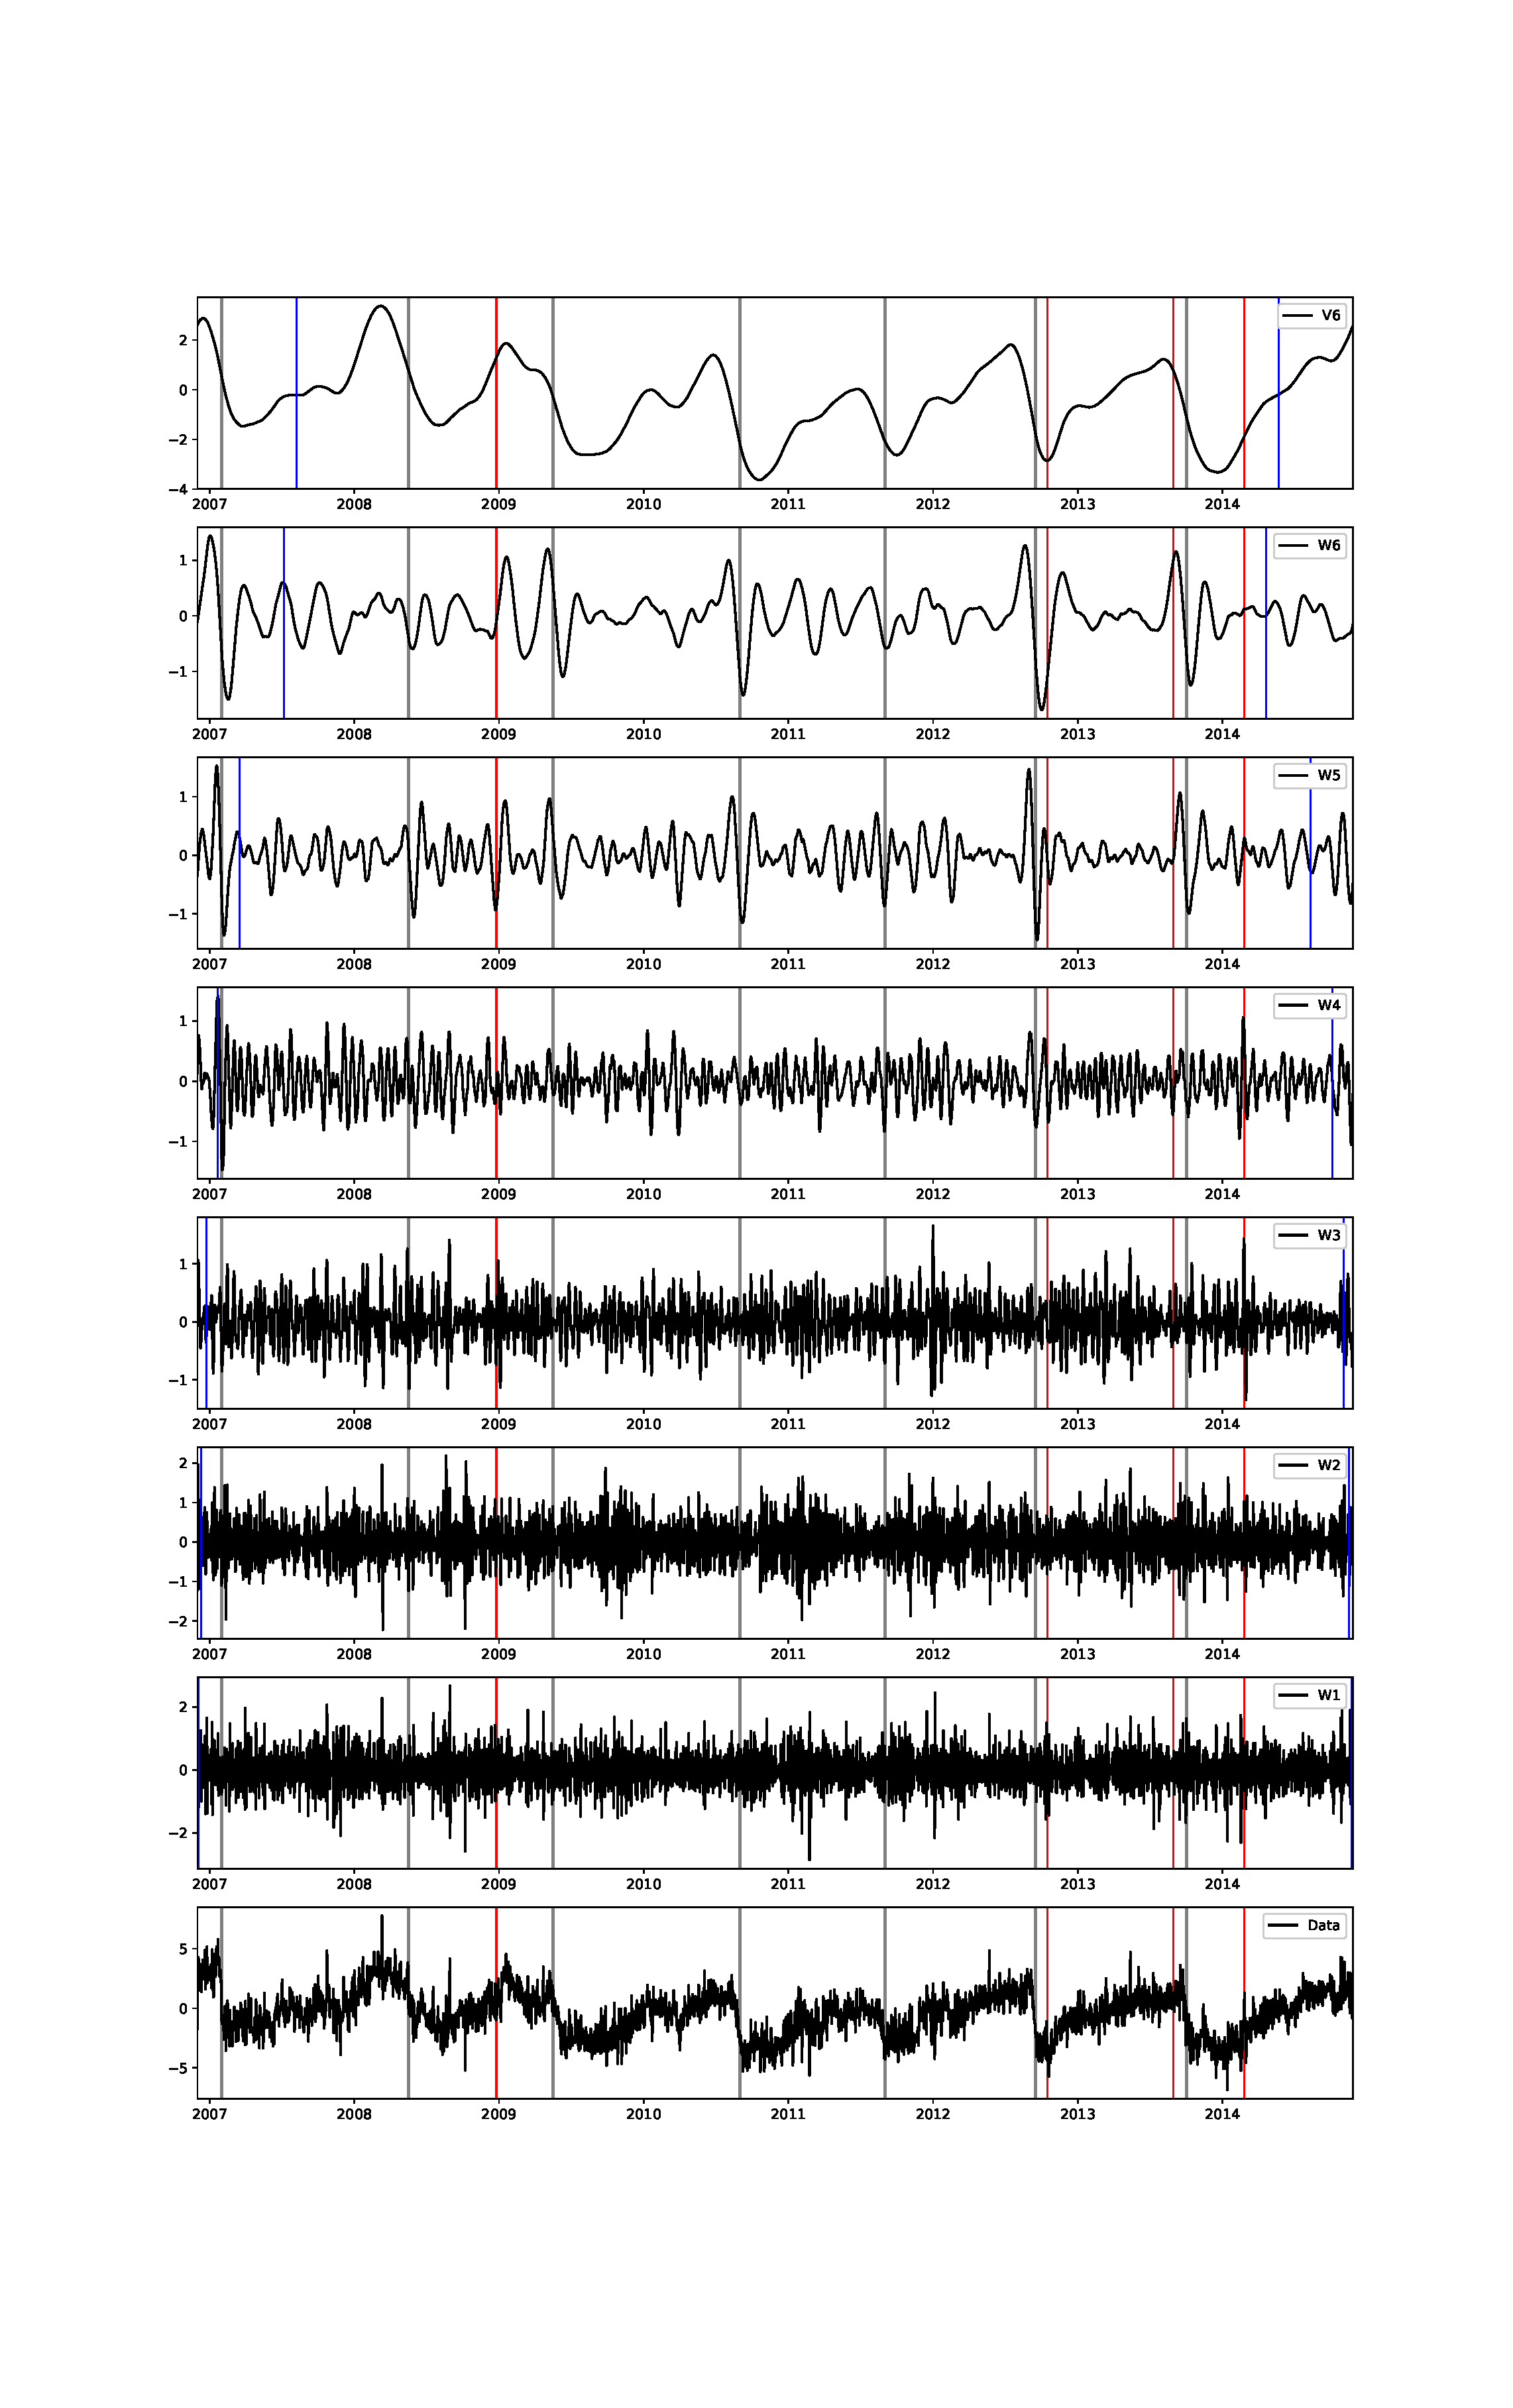
\includegraphics[width=300pt]{Figures/slowslip_results/Figure_3.eps}
\captionsetup{type=figure}
\captionof{figure}{Partial MODWT wavelet coefficients up to level 6.}
\end{center}

Finally, the 5\textsuperscript{th} and 6\textsuperscript{th} level details of the MRA are plotted with the cumulative number of tremor in Figure 19.4. Peaks corresponding to the August 2010, September 2012 and September 2013 ETS events can clearly be seen in both the 5\textsuperscript{th} and the 6\textsuperscript{th} level details. Peaks that could corresponds to the August 2011 ETS event, and a small inter-ETS event in March 2010, can also be seen in the 5\textsuperscript{th} level detail, but this is less obvious than for the other ETS events.

\begin{center}
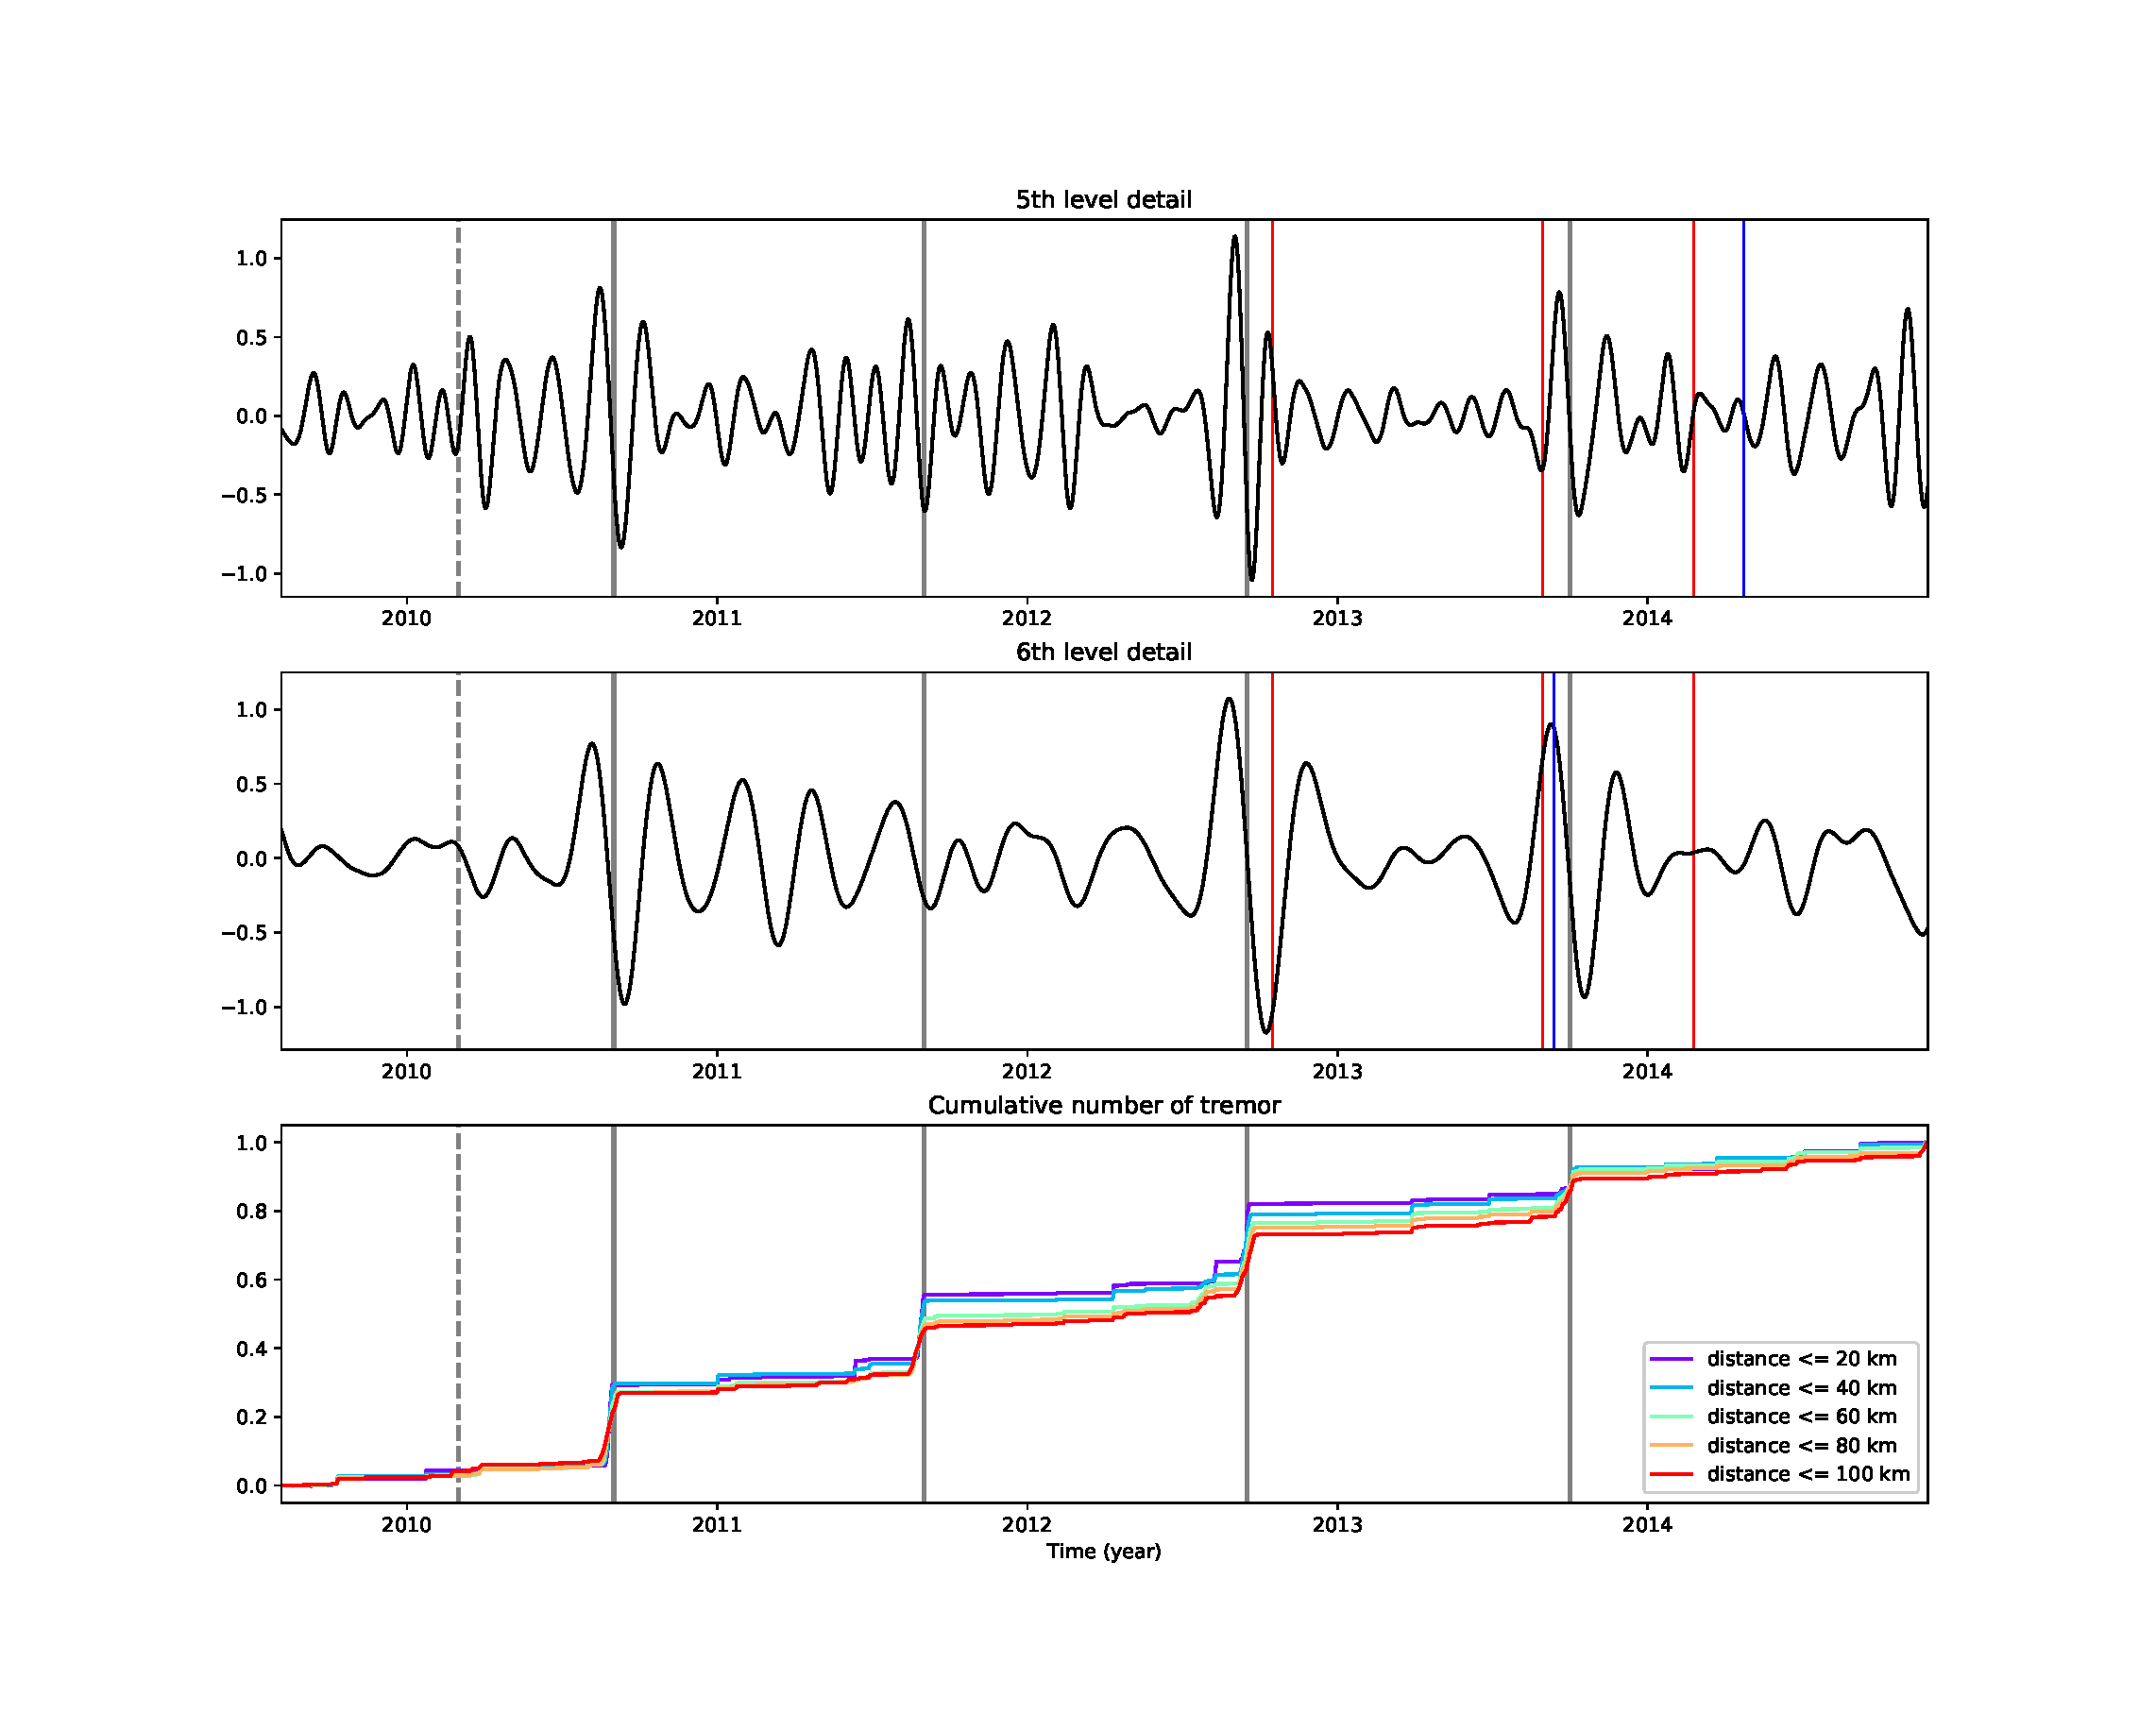
\includegraphics[width=300pt]{Figures/slowslip_results/Figure_4.eps}
\captionsetup{type=figure}
\captionof{figure}{5\textsuperscript{th} and 6\textsuperscript{th} level details of the partial MODWT analysis (top and middle panel), and cumulative number of tremor
recorded around the GPS station (bottom panel).}
\end{center}

We did a similar analysis with the GPS stations CLRS, CUSH, FRID, PNCL, PTAA, and SQIM, all located in the Olympic Peninsula, or on Vancouver Island, and we found similar results.

\chapter{Discussion and things to do}

Change point detection: Can we detect a big ETS event starting, and when can we detect it? Before it becomes obvious due to the tremor recordings? We could test other wavelets (Daubechies with extremal phase may be a good idea), or look at the wavelet variance (see paper by Eric Moulines - Kouamo et al., 2011, with correction of the mistake in Percival's paper).

\end{document}
